\PassOptionsToPackage{usenames,dvipsnames,table}{xcolor}
\documentclass[sigconf,balance,nonacm,authordraft]{acmart}

% packages
\usepackage[utf8]{inputenc}
\usepackage{amsmath}
\usepackage{commath}

\usepackage{graphicx}
\usepackage[caption=false,font=footnotesize]{subfig}
    
\usepackage{cleveref}

% algorithms
\usepackage{algorithm,algpseudocode}
 
% For syntax highlighting
\usepackage{specs}

\usepackage{soul}
\usepackage{booktabs}
\usepackage{multirow}
\usepackage[nolist,nohyperlinks]{acronym}
\usepackage{xspace}
\usepackage{url}

\usepackage{pgfplots}
\pgfplotsset{width=10cm,compat=1.9} 


% document
\begin{document}

% acronyms
\begin{acronym}
\acro{DSL}{Domain-Specific Language}
\acro{HPC}{High-Performance Computing}
\end{acronym}

% title and authors
\title{The Title of Your Work}

\author{Your Name}
\affiliation{%
  \institution{Department,\\University}
  \city{City} 
  \country{Country} 
  \postcode{Postal Code}
}
\email{Your Email}


\begin{abstract}
This is the abstract. Here, you should provide a short summary of the entire work. You should include the following elements: your research problem and objectives, your methods, your key results, and your conclusion. Aim for 150 to 300 words.
\end{abstract}

\keywords{Your, Keywords, Go, Here}

\maketitle

% % % % % % % % % % % % % % % % % % % % %
% 			INTRODUCTION
% % % % % % % % % % % % % % % % % % % % %
\section{Introduction}
\label{sec:intro}
This section serves as the introduction to the work and it is likely the second thing readers will focus on, after the abstract. This section should contextualize your work, introducing the topic and the expected results. Usually, it is also in this section that authors include a brief summary of the main contributions of the work.

Additionally, you can have several subsections for topics such as the problem statement, the motivation for this work, and also any needed background information for unfamiliar readers. These can also be made into their own sections that follow the introduction. The problem statement is a short description of the problem that your work addresses, identifying the gaps between the current state and the desired future state. The motivation should sell the importance of this work and the reader should understand what is the impact of solving the identified problem.

% % % % % % % % % % % % % % % % % % % % %
% 	    ACTIVITIES AND PLAN
% % % % % % % % % % % % % % % % % % % % %
\section{Activities and Plan}
\label{sec:activities}
In this section you should present the temporal evolution of the project. Include any relevant diagrams or charts, and list the finished tasks, possibly comparing them to the list of expected tasks.

% % % % % % % % % % % % % % % % % % % % %
% 			YOUR SOLUTION
% % % % % % % % % % % % % % % % % % % % %
\section{Your Solution}
\label{sec:solution}
In this section you will describe your work, both in form and function. That is, you should describe its structure/architecture, but also how it works, both internally and externally. Internally, any data structures and algorithms that you have used are relevant, especially if they were developed especially for this work. Externally, consider how an end-user would use your work.

Additionally, in this section you can also present the technical difficulties faced during the development, if and how they were overcome, and any limitations of the final product.

Artifacts such as code or API listings do not belong in this section. If they are important to the report and need to be included, they should be put in appendices at the end of the document.

% % % % % % % % % % % % % % % % % % % % %
% 			EXPERIMENTAL EVALUATION
% % % % % % % % % % % % % % % % % % % % %
\section{Experimental Evaluation}
\label{sec:evaluation}
In this section you can describe the experimental evaluation that your performed to evaluate your project.

\subsection{Experimental Setup}
In this subsection you present the setup you used to perform your tests. The benchmarks uses, the runtime system, the hardware, the methodology, and so on. This is needed for reproducibility purposes and for readers to understand how your work is more or less relevant in their own context.

\subsection{Experimental Results}
In this subsection you present the achieved results and you conduct an analysis of the experiments to see if the results obtained are what was expected according to your initial assumptions. If they are not, you are expected to understand and explain why.

% % % % % % % % % % % % % % % % % % % % %
% 			RELATED WORK
% % % % % % % % % % % % % % % % % % % % %
\section{Related Work}
\label{sec:rel}
In this section you can present other work that is relevant to your own research and development. Usually a short paragraph will explain how the other approach works and what are the main differences to your work, e.g., what problems were left open that you manage to solve or how you took a different approach and what are its pros and cons.

% % % % % % % % % % % % % % % % % % % % %
% 			CONCLUSIONS
% % % % % % % % % % % % % % % % % % % % %
\section{Conclusions}
\label{sec:conclusions}
In this section you present the main conclusions of your work in a summarized form. You can also present relevant future work on to to tackle current limitations and extend functionality.

% % % % % % % % % % % % % % % % % % % % %
%      USEFUL EXAMPLES (TO DELETE)
% % % % % % % % % % % % % % % % % % % % %
\section{Useful Examples}
\label{sec:examples}
This section, which you should delete later on, has examples on how to use some of Latex's most common features and environments.

\begin{figure}
    \begin{algorithmic}[1]
    \Function{MemoizedFunction}{input}
        \State $hash \gets \Call{HashFunction}{input}$
        \State $<found,output> \gets \Call{Lookup}{hash, input}$
        \If{$found=False$}
            \State $output \gets \Call{OriginalFunction}{input}$
            \State $\Call{Update}{hash, input, output}$
        \EndIf
        \State \Return $output$
    \EndFunction
  \end{algorithmic}
  \caption{This is the algorithm caption.}
  \label{alg:memoi}
\end{figure}

\Cref{alg:memoi} presents a basic algorithm using the \textit{algorithmic} environment for pseudo-code.

This is how you make an unumbered list:
\begin{itemize}
    \item This is the first item;
    \item This is the second item;
    \item This is the final item.
\end{itemize}

Whenever you cite someone else's work, you need to include a reference to the relevant source. This is how you make a citation~\cite{Michie1968}. You can also cite multiple sources at once like this~\cite{Strachey2000,Connors2000}. The references need to be present in the \textit{refs.bib} file.

\begin{figure}[t]
    \centering
    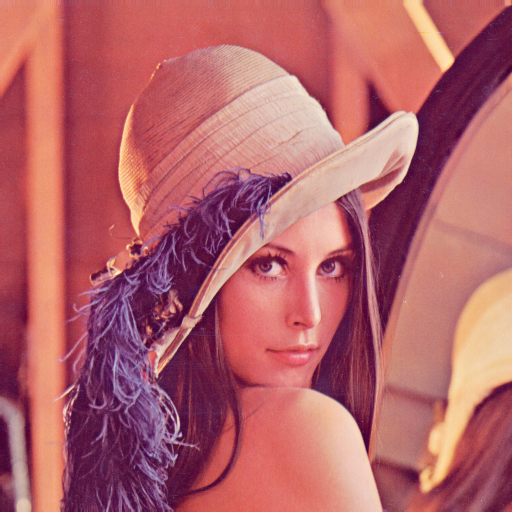
\includegraphics[width=0.8\columnwidth]{figures/lenna.png}
    \caption{This is the figure caption.}
    \label{fig:prof-motiv}
\end{figure}

\Cref{fig:prof-motiv} shows you how to include a figure. By default, Latex uses PNG or PDF formats for figures.

If you need to include equations, you can use Latex's excellent math environments. Here is a simple example of an equation:
\begin{equation}\label{eq:log}
    O(i, j) = c \times \log{(1+I(i, j))},
\end{equation}
where $c$ is a constant, $I$ is the input, $O$ is the output, and $i$ and $j$ are the image coordinates.

You can use the acronym package to help manage acronyms. The first time you use an acronym, its full form will be displayed, e.g., \ac{DSL} or \ac{HPC}. However, the following times, only the short version will be used, as in \ac{DSL} or \ac{HPC}. You can also use the plural form of acronyms, e.g., \acp{DSL}. The list of known acronyms is defined in the preamble of the document.

\begin{figure}[t]
 	\centering
	\lstinputlisting[boxpos=b,style=specs,language=C]{c/wrapper.c}
	\caption{This is the code caption.}
	\label{fig:code}
\end{figure}

If you want to include code, you can also do so by using the listings package. Here is an example of how to do it. \Cref{fig:code} presents an example of how to include source code.

Finally, tables can also be a good option to present data. \Cref{tab:table1} gives you an example of how to generate tables. Notice that the caption appears above the table, contrary to what happens with figures.

\begin{table}[b]
\caption{This is the table caption.}
\label{tab:table1}
\footnotesize
\begin{tabular}{lll}
\toprule
         & machine A                   & machine B                           \\
\midrule
CPU      & Intel Core i7-9700 CPU      & 2x Intel Xeon E5-2630 v3            \\
CPU Frequency& 3.00GHz                     & 2.40GHz                             \\
RAM      & 16GB DDR4                   & 128GB                               \\
OS       & Ubuntu 20.04 LTS            & Ubuntu 16.04 LTS                    \\
Compiler & GCC 9.3                     & GCC 7.3                             \\
libm     & v2.31                       & v2.23                               \\
libomp   & v4.5                        & v4.5                                \\
\bottomrule
\end{tabular}
\end{table}

% % % % % % % % % % % % % % % % % % % % %
% 			ACKNOWLEDGMENTS
% % % % % % % % % % % % % % % % % % % % %
\section*{Acknowledgments}
The author would like to acknowledge \ldots

% % % % % % % % % % % % % % % % % % % % %
% 			BIBLIOGRAPHY
% % % % % % % % % % % % % % % % % % % % %
\bibliographystyle{ACM-Reference-Format}
\bibliography{refs}

\end{document}
